\documentclass[french]{article}
\usepackage[T1]{fontenc}
\usepackage[french]{babel}
\usepackage[utf8]{inputenc}
\usepackage{a4wide}
\usepackage{amssymb}
\usepackage{amsmath}
\usepackage{listings}
\usepackage{graphicx}

% --JUGEMENTS-- %
\newcommand{\jugementPointeur}{
        \dfrac{\sigma \vdash id : \tau}
              {\sigma \vdash *id : \tau, \pi} \text{où }\pi \text{ est la marque.}\\
        \text{Par suite, } \tau_r \text{ est l'environnement de type et de marque.}\\
        \text{Les jugements de typages sont alors inchangés, simplement on peut remplacer}\\
        \text{pour les variables id par *id en suivant le typage ci-dessus.}
        }

\newcommand{\jugementElseOpt}{
        \dfrac{\sigma \vdash E : \text{bool} \hspace*{10pt} \sigma, \tau_r \vdash \text{BLOC} : \text{void}}
              {\sigma, \tau_r \vdash \text{if } E \text{ BLOC} : \text{void}, []}
        }

\newcommand{\jugementTernaire}{
        \dfrac{\sigma \vdash E : \text{bool} \hspace*{10pt} \sigma \vdash E_1 : \tau \hspace*{10pt} \sigma \vdash E_2 : \tau }
              {\sigma \vdash (E \text{ ? } E_1 : E_2) : \tau}
        }

\newcommand{\jugementLoop}{
        \dfrac{\sigma, \tau_r \vdash \text{BLOC} : \text{void}}
              {\sigma, \tau_r \vdash \text{loop} \text{ BLOC} : \text{void}, []}
        }
\newcommand{\jugementLoopId}{
        \dfrac{id::\sigma, \tau_r \vdash \text{BLOC} : \text{void}}
              {\sigma, \tau_r \vdash \text{define id : loop} \text{ BLOC} : \text{void}, []}
        }

\newcommand{\jugementIncrementPost}{
        \dfrac{\sigma \vdash id : \text{Int}}
              {\sigma \vdash \text{id}++ : \text{Int}}
        }

\newcommand{\jugementIncrementPre}{
        \dfrac{\sigma \vdash id : \text{Int}}
              {\sigma \vdash ++\text{id} : \text{Int}}
        }

\begin{document}


\title{\textbf{Traduction des Langages}}
\author{Quentin \textsc{Fraty}\\
        Nathan \textsc{Maillet}}
\date{}

\maketitle

% Transversale (?)
% !! Penser a traiter les évolutions des AST !!
% Justifications pertinentes et complètes sur l'evolution de la structure des AST.
% Comparaison avec d'autres choix de conception
% Effacer les lignes de ce message UNIQUEMENT lorsque qu'elles ont été traitées

\section{Introduction}
% Bonne description du sujet et des points abordés dans la suite du rapport
% pas de copier/coller du sujet !!
% Effacer les lignes de ce message UNIQUEMENT lorsque qu'elles ont été traitées
\paragraph{Dans la continuité des cours / TDs / TPs effectués en rapport avec le concept de Traduction des Langages, un projet de développement de compilateur
a été réalisé. Le langage d'origine choisi fut le Rat, car étant largement limité en termes d'opérations réalisables dans un programme.\\
Le langage cible, quand à lui était un pseudo langage assembleur pouvant être exécuté directement à travers un programme spécialisé.}
\paragraph{Comme nous allons le voir tout au long de ce rapport, une grande variété de fonctionnalités ont été ajoutées au langage Rat,
avec comme objectif de le rendre plus complet, et plus proche des langages bas niveau manipulés aujourd'hui (Rust, C).\\
Notamment, voici les différentes fonctionnalités implémentées et opérationnelles, qui seront abordées:}
\begin{itemize}
        \item Ajout des pointeurs, et accès par référence à des variables.
        \item Ajout du côté optionel au bloc else d'une conditionnelle.
        \item Ajout des expressions ternaires.
        \item Ajout des boucles `à la Rust'.
\end{itemize}
\paragraph{Voici ensuite les fonctionnalités non demandées implémentées:}
\begin{itemize}
        \item Ajout de la surcharge de fonctions (même nom, différents types de paramètres).
        \item Ajout d'instructions pour l'incrémentation rapide (v++, ++v, v+=42).
        \item Ajout d'une backtrace en cas d'erreur.
\end{itemize}
\section{Mutation de \emph{tds.ml} en \emph{mtds}}
% Rq : mtds a pour vocation de généraliser tds
%      plutôt que de changer tds.ml pour inclure les ptrs et
%      galérer dans le cas où on veut revenir en arrière ou modifier
%      les identifiants a l'avenir (casts, expliciter les kinds -btw, ça existe ? ça marche comment en cpp ?)
%      il n'y aura pas besoin de changer mtds
%      -> cela nous a été utile car on a changé de stratégie pour les ptrs
%      mtds n'est pas contraint par une structure de monade car je ne vois pas l'intérêt dans le monde OCaml pré version 5...
% Effacer les lignes de ce message UNIQUEMENT lorsque qu'elles ont été traitées
\paragraph*{La première étape avant de se lancer sur le projet était de modifier \emph{tds.ml} afin de ne plus le modifier,
même si par la suite nous voulions modifier notre raisonnement, comme par exemple sur les pointeurs.}
\subparagraph*{\emph{mtds.ml} a donc pour but de généraliser \emph{tds.ml}. Nous sommes donc passés d'Identifiants \emph{string}
en \emph{'a}, ce qui explicite l'aspect monadique de la tds sans pour autant la contraindre, ce qui aurait été un apport négligeable en OCaml 4.}

\section{Pointeurs}
% Explications pertinentes et complètes sur leur traitement (sans...). Comparaison avec d’autres choix de conception.
% Ne pas oublier les jugements de typage !
% Rq : question cruciale : est-ce que int *a c'est ( int * ) a ou int ( *a ) ? 
%         choix : int ( *a ), on traite ( *a )
%         comme l'indentifiant, constitué d'un marqueur : * et d'un symbole/identifiant : a 
% Effacer les lignes de ce message UNIQUEMENT lorsque qu'elles ont été traitées

\section{Bloc else optionnel}
% Explications pertinentes et complètes sur leur traitement (sans...). Comparaison avec d’autres choix de conception.
% Ne pas oublier les jugements de typage !
% Effacer les lignes de ce message UNIQUEMENT lorsque qu'elles ont été traitées
\paragraph*{Grâce à la façon choisie initialement pour traiter les blocs conditionnels, il fut assez simple d'implémenter cette fonctionnalité.
En effet, lors du parsing, il suffit de créer un \textit{AstSyntax.Conditionnelle} avec un bloc else vide, et de le traiter comme un bloc conditionnel classique.
Le typage est inchangé, et le code produit est le même que si le bloc else était présent.}
\paragraph*{Cette solution permet de minimiser la redondance de code, et de ne pas avoir à traiter le bloc else comme un cas particulier, avec comme seul bémol
que la passe de génération de code rajoute dans tous les cas un label pour le else, qu'il soit vide ou non. Cela n'a aucun impact sur l'exécution du programme.}
\paragraph*{Au niveau du jugement de typage, dans la mesure où le bloc else est vide, celui-ci peut être résumé comme suit:}
\[\jugementElseOpt\]

\section{Conditionnelle ternaire}
% Explications pertinentes et complètes sur leur traitement (sans...). Comparaison avec d’autres choix de conception.
% Ne pas oublier les jugements de typage !
% Effacer les lignes de ce message UNIQUEMENT lorsque qu'elles ont été traitées
\paragraph*{Cette fonctionnalité ajoutée au langage Rat a nécessité de créer un nouveau type d'expression, \textit{AstSyntax.Ternaire}.
Tout d'abord, il a fallu modifier la grammaire pour accepter cette nouvelle expression~:}
\subparagraph*{Au niveau du lexer, il a fallu ajouter le symbole \texttt{?} et \texttt{:} dans la liste des symboles à accepter. Au niveau du parser, il a fallu ajouter une règle pour accepter cette nouvelle expression~:}
\,% les listings sont kssé
\begin{lstlisting}
| PO e1=e QMARK e2=e COLON e3=e PF  {Ternaire (e1,e2,e3)}
\end{lstlisting}

\paragraph*{Ensuite, les différentes passes du compilateur ont successivement vérifié les choses suivantes~:
\begin{itemize}
        \item La conformité des identifiants utilisés dans les trois expressions de la conditionnelle ternaire.
        \item Le fait que la premiere expression soit bien booléenne, et que les deux autres soient de même type. Cela peut être résumé par le jugement de typage suivant~:
\end{itemize}}
\[\jugementTernaire\]
\paragraph*{Enfin, la génération du code associé à un ternaire se rapproche à celui d'une instruction conditionnelle, 
dans la mesure où la valeur mise en sommet de pile est celle de l'une des deux expressions~: l'utilisation de jump est alors nécessaire.}
\,
\begin{lstlisting}
| AstType.Ternaire(e1, e2, e3) -> 
      let labElse = getEtiquette ()
      and labEndIF = getEtiquette () in
      ast_to_tam_expression e1
      ^ jumpif 0 labElse
      ^ ast_to_tam_expression e2
      ^ jump labEndIF
      ^ label labElse
      ^ ast_to_tam_expression e3
      ^ label labEndIF
\end{lstlisting}

\section{Loop à la Rust}
% Explications pertinentes et complètes sur leur traitement (sans...). Comparaison avec d’autres choix de conception.
% Ne pas oublier les jugements de typage !
% Rq : Problème de la pile a évoqué
% Effacer les lignes de ce message UNIQUEMENT lorsque qu'elles ont été traitées
\paragraph*{Les loop à la rust sont une extension du langage Rat qui permet de créer des boucles infinies,
avec la possibilité de les casser à l'aide du mot clé \texttt{break} 
et de terminer prématurément une itération à l'aide du mot clé \texttt{continue}.}
\paragraph*{TODO:\@ grammaire}
\paragraph*{Comme nous allons le voir, toute la complexité des boucles à la rust est liée à la gestion des labels, qui est exclusivement gérée par la passe de gestion d'identifiants.\\
Tout d'abord, il a été choisi de créer un nouveau type de données insérables dans la table des symboles.}
\subparagraph*{En effet, il est nécessaire de stocker les informations liées à une boucle pour pouvoir la terminer, ou la recommencer
lorsqu'un break ou continue est utilisé.\\
Cependant, et ce comme énoncé dans le sujet, il fallait donner la possibilité à l'utilisateur d'imbriquer des fonctions de même label.\\
Pour ce faire, ce nouvel élément de la TDS associe à un label une InfoBoucle, qui contient en réalité une liste d'informations associées à ce label.\\
Cela permet de prendre en compte le cas où deux boucles de même label sont imbriquées, et de pouvoir les distinguer. \\} % Espacement voulu
\subparagraph*{Un deuxième choix de conception réside dans le choix des informations stockées dans la TDS pour les boucles.\\
Tout d'abord, à toute boucle est associé un identifiant pour la TDS:\@soit celui donné par l'utilisateur, soit un identifiant uniqué généré par le compilateur
de manière analoque à la génération de labels lors de la passe de génération de code.}
\,
\begin{lstlisting}
let giveID = 
  let num = ref 0 in
  fun () ->
    num := (!num)+1 ;
    "id"^((string_of_int (!num)))
\end{lstlisting}
\paragraph{Ensuite, l'information associée à une boucle est le couple (label de début, label de fin), qui sont générés par le compilateur à partir du label précédent. \\
Ainsi, lorsque deux boucles de même label sont utilisées, l'infoboucle associée au label est une liste de couples 
(label de début, label de fin), dont la tête est le couple associé à la plus imbriquée.
Grâce à la récursivité du langage fonctionnel, il est possible de récupérer le label de début/fin de la boucle la plus imbriquée de manière efficace,
ce qui est la logique choisie pour le break et le continue.}
\subparagraph{De plus, il fallait donner la possibilité à l'utilisateur de ne pas utiliser de labels pour les loops, break et continue. Le comportement
choisi devait alors être que tout break / continue aurait un effet sur la boucle courante, et dans le cas d'imbrication de boucles, celle la 
plus imbriquée.\\
Pour pouvoir implémenter cela, il a été choisi de \textit{décorer l'arbre} avec l'infoboucle associée à la boucle courante pour pouvoir associer au break / continue
la bonne boucle.}
\paragraph{Suite à cette passe, celle de typage est comparativement triviale, dans la mesure où celle-ci revient à une analyse
du typage d'un bloc. Voici les jugements de typage associé~:}
 \[\jugementLoop \text{ et } \jugementLoopId\]
\paragraph{La passe de placement mémoire, de manière analogue, revient à analyser le placement mémoire des variables du bloc de la boucle.}
\paragraph{En revanche, la passe de génération de code s'avéra poser des difficultés que nous n'avions pas anticipé. En effet, chaque itération de boucle doit
écrire ses variables locales au même endroit, ce qui pose des problèmes lorsqu'un break ou un continue sont utilisés: alors que le TantQue
implémenté en Rat assurait l'exécution entière de son bloc courant avant de se finir, ce n'est pas le cas de la boucle à la Rust. \\
Ainsi, en imaginant qu'un break prématuré puisse faire 'éviter' une déclaration de variable (et donc un push de la pile), il s'avérait nécessaire
d'avoir le nombre de déclarations dans la boucle actuelle en tant que paramètre hérité (décoration d'arbre). Cependant même avec une telle chose, 
le cas d'imbrication de boucle ne semblait pas traitable, dans la mesure où un break peut aussi faire sortir d'une boucle moins imbriqué, comme dans 
l'exemple suivant:}

\, % les listings sont kssé
\begin{lstlisting}
        main {
                int x = 3;
                define l : loop {
                        x++;
                        loop {
                                int y = 5;
                                break l;
                                bool z = true;
                        };
                        rat r = [3/2];
                };
        }
\end{lstlisting}
\paragraph{Ici, il faudrait \textit{se rappeler} au niveau du break l que cela revient à pop 1, et pas 2 ou 3 qui serait obtenu si on prenait toutes les déclarations réalisées.\\
N'ayant pas de solution simple à ce problème et par manque de temps, il a été choisi de ne \textbf{pas} pop le contexte d'une boucle en cas de break ou continue.
Ce choix, bien que semblant fonctionner, peut poser des problèmes de pile si un utilisateur venait à réaliser un \textit{continue inconditionnel} dans une boucle, 
ce qui dupliquerait le contexte à chaque itération.}

\section{Surcharge de fonctions}
% Explications pertinentes et complètes sur leur traitement (sans...). Comparaison avec d’autres choix de conception.
% Effacer les lignes de ce message UNIQUEMENT lorsque qu'elles ont été traitées

\section{Incréments}
% Explications pertinentes et complètes sur leur traitement (sans...). Comparaison avec d’autres choix de conception.
% Ne pas oublier les jugements de typage !
% Effacer les lignes de ce message UNIQUEMENT lorsque qu'elles ont été traitées
\paragraph{Il a été choisi d'implémenter dans le langage Rat de nouvelles fonctionnalités qui puissent êtres traitées au niveau du parseur. C'est pourquoi
l'incrémentation comme en C (variable++ et ++variable) a été partiellement ajoutée: contrairement à C, ces deux éléments sont considérés comme
des instructions à part entière, ce qui limite leur intérét à celui d'un compteur. Voici les lignes associées dans le fichier Parser~:}
\,
\begin{lstlisting}
| PLUS PLUS n=r PV 
{Affectation (n,Binaire (Plus,Identifiant n,Entier 1))}
| n=r PLUS PLUS PV 
{Affectation (n,Binaire (Plus,Identifiant n,Entier 1))}
\end{lstlisting}
De manière similaire, l'opérateur '+=' a été ajouté au langage Rat, et ce grâce à une transformation directement dans le parseur:
\begin{lstlisting}
| n=r PLUS EQUAL e1=e PV 
{Affectation (n,Binaire (Plus,Identifiant n,e1))}
\end{lstlisting} 
\paragraph{Ainsi, dans la mesure où ces instructions sont `converties' en combinaisons d'éléments simples compris par notre compilateur, aucune passe n'a
à être adaptée pour prendre en compte ces opérations.}
\section{Affichage des erreurs}
% Explications pertinentes et complètes sur leur traitement (sans...). Comparaison avec d’autres choix de conception.
% Effacer les lignes de ce message UNIQUEMENT lorsque qu'elles ont été traitées
\paragraph{La génération de backtrace est la dernière fonctionnalité optionnelle que nous avons ajouté à notre compilateur Rat. \\
Celle-ci permet à un développeur de savoir précisément à quelle ligne de quel bloc se situe l'erreur empêchant la compilation. 
Voici par exemple la backtrace générée:}
\begin{center}
        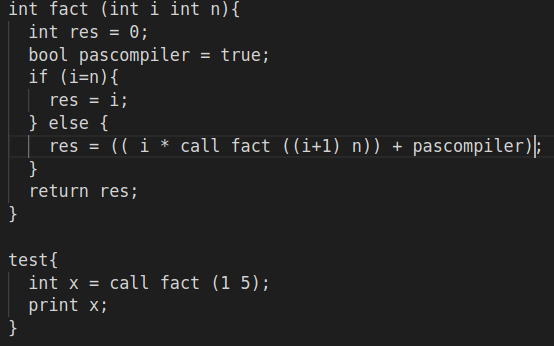
\includegraphics[scale=0.4]{code_compile_pas.png}
        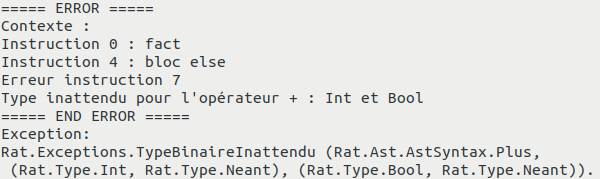
\includegraphics[scale=0.4]{backtrace.png}
\end{center}
\paragraph{
Même si cette fonctionnalité reste au niveau de preuve de concept (mot-clé `fonction' non utilisé, numérotation commençant à 0), celle-ci
permet à un utilisateur développant un plus gros programme de retrouver rapidement dans son code l'instruction fautive. \\
Ce résultat utilise le concept de décoration d'arbre, comme réalisé pour d'autres fonctionnalités: après la passe de gestion des identifants,
à chaque instruction est rajouté un contexte. Il s'agit d'une liste de couple (numéro de ligne, nom du bloc) représentant avec précision la localisation
de chaque instruction dans le code. Ainsi, toute erreur levée fait désormais appel à notre fonction `afficher\_erreur' prenant en paramètres
un contexte,une exception et son numéro de ligne, et l'affichant comme montré précédemment.}
\section{Conclusion}
% Bon recul sur les difficultés rencontrées et améliorations éventuelles
% Améliorations éventuelles :
% On n'autorise pas les fonctions d'ordre supérieur avec les pointeurs mais
% attention a gérer le LB !!
% On autorise les pointeurs dans les paramètres mais pas en retour
% Effacer les lignes de ce message UNIQUEMENT lorsque qu'elles ont été traitées

\end{document}
